% EmoH3 — workshop paper, submission-ready skeleton
% Compile: pdflatex paper_emoh3.tex (uses only standard packages)
\documentclass[10pt,twocolumn]{article}
\usepackage[utf8]{inputenc}
\usepackage[margin=1in]{geometry}
\usepackage{amsmath,amssymb}
\usepackage{booktabs}
\usepackage{graphicx}
\usepackage{xcolor}
\usepackage{caption}
\usepackage{hyperref}
\usepackage[numbers]{natbib}

\title{\textbf{Emotion-Control Evaluation Is Not Invariant: Judge, Option Order and\\ Judged Frame Span Flip 11--58\% of Verdicts on MiniMax H3}}

\author{Anonymous}
\date{}

\begin{document}
\maketitle

\begin{abstract}
Controllable generation of a specific anime character in a desired emotional state is a core
requirement for AI-assisted animation production, yet portrait-reference (Ref2VA) video
generators such as MiniMax H3 tend to lock the output to the \emph{reference's} emotion,
suppressing prompt-specified targets---most severely for negative and subtle emotions. Studying this
on MiniMax H3 (33B, joint video+audio, 8$\times$H100), we find that the binding constraint is the
\emph{measurement}, and we quantify it along three orthogonal, essentially free protocol choices.
\textbf{(i) Judge}: across four open Qwen judges (7B--32B, four releases spanning three generations) none validates on more
than 1/17 taxonomy-relevant known emotions, none recognizes any negative emotion, and on the same
clip-configs all four agree on only 23/77 (Fleiss $\kappa{=}0.38$; pairwise 41.6--71.6\%, each on its own common set).
\textbf{(ii) Option order}: merely reversing the 15 answer options flips 17/88 and 10/88 verdicts on
identical frames under greedy decoding, while a duplicate run of one variant reproduces 88/88 word-identically. \textbf{(iii) Temporal
coverage}---the largest \emph{within-judge} axis and the only one with significant model-side effects (a change of judge across
capability tiers moves more, 58\%): our protocol, like much practice, judged 8
frames from the first second of each 5.2\,s clip; re-judging the whole clip changes 32/97, 32/97 and 34/97
verdicts under three judges (Cohen $\kappa{=}0.48$--$0.57$), predominantly
neutral$\rightarrow$committed, raising target-hit rates on the base arm from 8/34 to 16/34 (exact
McNemar $p{=}0.021$) and on the LoRA arm from 13/63 to 23/63 and 20/63 to 33/63 ($p{=}0.002$, $0.001$). This
reverses our own conclusions: the baseline ``failures'' become successes and the control premise
``base never expresses sad'' (0/6) becomes 2/6, so we \emph{retract} our task-level claim for a
reference-conditioned LoRA and report it only as the case study whose evaluation flips. What survives
all scorings is the mechanism---the LoRA suppresses reference-emotion tracking (base 5/8, 4/8, 3/8,
4/8 vs 2/8 in every condition)---and it is underpowered ($n{=}8$). Frown-type targets remain
untestable with the weakest judge, and a 768$^2$ ablation rules out a resolution-mismatch
explanation. Until judges are validated on the emotions they score and protocols fix temporal
coverage, reported emotion-control gains are not interpretable. All verdicts, frames and scripts
are released.
\end{abstract}

\section{Introduction}
Character-consistent, emotion-controllable video generation is central to animation and
virtual-content workflows: given a character's portrait (reference) and a natural-language
instruction (``She smiles joyfully.''), a generator should animate \emph{that} character
\emph{in that state}. Recent portrait-reference video generators---e.g.\ MiniMax H3's Ref2VA
mode~\cite{minimax2025}---condition synthesis on both a text prompt and a reference image and
are remarkably good at preserving identity. In practice, however, we observe a strong
\emph{reference-emotion dominance}: the generated video tends to reproduce the reference's
expression, and prompt-specified targets that disagree with the reference are often ignored,
especially when the target is negative or subtle (sad, worried, relieved, angry).

This paper studies whether this limitation can be addressed on a single 8$\times$H100 node with
an open 33B video+audio model. We make no claim of state-of-the-art generation quality; instead
we contribute an \emph{honest, reproducible} account of (a) how unreliable emotion-control
evaluation currently is, (b) a training intervention that yields a measurable, controlled
improvement, and (c) a clearly bounded failure region.

Our findings rest on a small but carefully controlled protocol:
\begin{itemize}
\item \textbf{Evaluation.} Eight emotion-transfer tasks (e.g.\ neutral$\rightarrow$sad,
angry$\rightarrow$happy), each pairing a reference portrait with a target-emotion prompt.
Generated 124-frame videos are judged by Qwen2-VL-7B~\cite{qwen2vl2024}, an open vision-language
model, with a fixed anime emotion taxonomy. Every configuration is run under $\ge$2 seeds and
$\ge$2 step counts; the judge reads 4 or 8 uniformly sampled frames.
\item \textbf{Method.} We add \emph{reference conditioning} to the training objective: the
reference image is encoded exactly as at inference and injected as clean conditioning rows into
the packed sequence (matching Ref2VA's layout), and training data include cross-emotion pairs
(reference shows emotion A, target video shows emotion $B\neq A$) so the model learns to let the
prompt override the reference.
\item \textbf{Findings.} (1) Base MiniMax H3 succeeds on 1/8 tasks at 8 inference steps, and this
``failure'' is partly a sampling artifact: at 16 steps the base model surfaces positive emotions.
(2) The instrument is unstable along three essentially free axes: judge identity (four open Qwen
judges agree on only 23/77 configs, Fleiss $\kappa{=}0.38$), answer-option order (reversing it flips
17/88 and 10/88 verdicts), and judged frame span (judging the whole clip instead of its first second
changes 32/97, 32/97 and 34/97 verdicts under three judges, with the only significant model-side
effects, McNemar $p{\le}0.021$ in three of six arm$\times$judge cells).
(3) We therefore \emph{retract} our earlier task-level claim for a reference-conditioned LoRA: judged
over the whole clip the baseline's ``failures'' become successes and its ``never-sad'' control (0/6)
becomes 2/6, so no measurable task-level improvement survives. What survives every scoring is the
mechanism---suppression of reference-emotion tracking (base 5/8, 4/8, 3/8, 4/8 vs v3 2/8 in all four
judge$\times$frame-span conditions, Sec.~\ref{sec:mech}; underpowered, $n{=}8$). (4) Frown-type
negatives (worried, angry) remain unsolved under all interventions---including a 768$^2$
training-resolution variant that refutes the ``layout mismatch'' hypothesis.
\end{itemize}

\section{Related Work}
\textbf{Video generation.} Open video diffusion transformers (CogVideoX~\cite{cogvideox2024},
HunyuanVideo~\cite{hunyuan2024}, Wan2.1~\cite{wan2025}) and closed systems
(Sora~\cite{sora2024}) have driven rapid progress; MiniMax H3~\cite{minimax2025} is notable for
joint video+audio generation with reference-image (Ref2VA) and first/last-frame (FL2VA)
conditioning, and it is the model we study.

\textbf{Character animation and personalization.} Character-consistency methods condition on a
reference image via cross-attention adapters (AnimateAnyone~\cite{animateanyone2023},
StableAnimator~\cite{stableanimator2024}) or image-prompt adapters
(IP-Adapter~\cite{ipadapter2023}). In the tuning-free setting these achieve strong identity
preservation but, as we show, weak \emph{emotion} control, since the reference encodes expression
as well as identity. Parameter-efficient fine-tuning (LoRA~\cite{lora2021},
DreamBooth~\cite{dreambooth2022}) adapts a base model to a subject or style; we use LoRA for
emotion \emph{behavior} rather than subject identity.

\textbf{Emotion and expression control.} A large literature controls facial expression in
talking-head and image-animation models; fewer works target \emph{full-body character} emotion in
video diffusion from a single portrait. Our focus is complementary: we treat emotion as a
first-class conditioning variable in an open portrait-to-video model and measure, adversarially
(by choosing references whose emotion disagrees with the target), how controllable it actually is.

\textbf{Automatic evaluation of generative video.} Human studies are costly; recent work
increasingly uses strong vision-language models as judges. We adopt
Qwen2-VL-7B~\cite{qwen2vl2024} with a fixed emotion taxonomy and, crucially, \emph{sweep its
inputs} (frame count, seed, steps) to expose evaluation instability---a methodological point we
believe applies beyond our task.

\section{Background: MiniMax H3 Ref2VA}
MiniMax H3 is a 33B-parameter rectified-flow video+audio diffusion transformer. In Ref2VA mode the
input is $[\text{text} \mid \text{reference blocks} \mid \text{target audio} \mid
\text{target video}]$ packed into one sequence with per-row rotary positions; the reference image
is encoded by the video autoencoder into a single-frame latent, patched into conditioning video
rows, and fed clean at a pinned timestep (0.999). At generation the target rows are denoised while
conditioning rows stay fixed---so the reference has direct attention access to every target token.
This makes the reference's emotional content a strong prior; our training intervention (Sec.~5)
mirrors the same layout so the LoRA can learn to modulate it.

We run all experiments on a single 8$\times$H100 node (80\,GB each), FSDP2 for inference and
DeepSpeed-ZeRO-3 for training; video 768$\times$768$\times$124, 16 inference steps (Sec.~4.2), and
LoRA rank 16 / alpha 32 on attention projections.

\section{Evaluation Protocol and Its Pitfalls}
\subsection{Tasks, judge, and protocol}
We define eight emotion-transfer tasks covering positive, negative, and subtle targets
(Table~\ref{tab:tasks}). Each uses a distinct character's portrait as reference and a
target-emotion prompt (e.g.\ x02: neutral portrait + ``She looks sad.''). For each clip we sample
4 or 8 frames, spaced evenly over the first second of each 5.2\,s, 124-frame clip---covering 19\% of
the clip, the segment where the reference portrait's expression is most likely to persist---and ask
Qwen2-VL-7B
($\text{do\_sample}=\text{False}$) to classify the emotion from
a fixed \textbf{15-class taxonomy} (the 12 released classes plus joyful, worried, cheerful) with a
confidence score. A task \emph{succeeds} iff the judged emotion equals the target, with one stated
synonym rule: joyful and cheerful count via their in-taxonomy synonym \emph{happy}. The judge never
emits 11 of its 15 classes (incl.\ all of worried/relieved/angry) across the 88 clip-configs, so those
targets are \emph{untestable} with this judge (Sec.~4.2). The judged window is itself a measured
limitation: it samples only the opening of each clip, and Sec.~4.1 shows that re-extracting frames
over the \emph{whole} clip flips up to a third of verdicts. Full-span frames are produced by
\texttt{extract8\_full.py}, re-scored with the identical protocol by \texttt{judge\_frameset.py},
and analyzed by \texttt{analyze\_framespan.py} (all released).

\begin{table}[t]
\centering\small
\caption{Eight emotion-transfer tasks.}
\label{tab:tasks}
\begin{tabular}{@{}lll@{}}
\toprule
ID & Reference $\rightarrow$ target & Prompt \\
\midrule
x01 & neutral $\rightarrow$ joyful & She smiles joyfully.\\
x02 & neutral $\rightarrow$ sad & She looks sad.\\
x03 & angry $\rightarrow$ happy & She laughs happily.\\
x04 & joyful $\rightarrow$ worried & She frowns worriedly.\\
x05 & amused $\rightarrow$ surprised & She looks surprised.\\
x06 & anxious $\rightarrow$ relieved & She smiles with relief.\\
x07 & sad $\rightarrow$ cheerful & She giggles cheerfully.\\
x08 & curious $\rightarrow$ angry & She looks angry.\\
\bottomrule
\end{tabular}
\end{table}

\subsection{Result 1: evaluation is unstable --- steps, seeds, frames flip verdicts}
Four failure modes of a naive protocol, quantified per clip in the release:
\begin{itemize}
\item \textbf{Inference steps.} Base model, x01 (neutral$\rightarrow$joyful): judged \emph{neutral}
at both 8 and 16 steps under a fixed 8-frame judge. A step flip we reported in an earlier protocol
did \emph{not} replicate at fixed frame count---that comparison also changed the judge frame count
and taxonomy and was confounded. We find no clean step effect.
\item \textbf{Sampling seed.} LoRA-v3, x02 (neutral$\rightarrow$sad): seed 42
$\rightarrow$ neutral; seed 1234 $\rightarrow$ \textbf{sad (80)}, under both the 12- and 15-class
judges. Same weights and prompt, flipped verdict.
\item \textbf{Judge frame count.} 4/88 clip-configs flip between 4 and 8 frames (e.g.\ base
x03 16s: neutral at 4fr, happy:90 at 8fr; v1 x07: happy at 4fr, neutral at 8fr).
\item \textbf{Judge choice.} Qwen2.5-VL-7B (same protocol) reads the decisive v3 x02 clip
\emph{neutral:85} and Qwen3-VL-32B \emph{worried:85}, where Qwen2-VL says sad:80; the strongest
judge (Qwen3.8-27B) says sad:82 (reproduced 85/82), and base x02 is neutral under all four. Verdicts
are not judge-invariant, and the disagreement is \emph{not} explainable by judge competence: the
corroborating Qwen3.8-27B mislabels a clear crying portrait fearful:85, so all four judges fail the
negative-emotion check (0/5).
\item \textbf{Temporal frame span} (the largest within-judge axis, and the only one yielding significant model-side effects): the 8 judged frames
covered only the first second of each 5.2\,s clip ($\sim$19\%); re-extracting 8 frames spanning the
whole clip, changing nothing else (same judge, same 15-class forced choice, same prompt, greedy),
flips 32/97 verdicts for Qwen2-VL (self-agreement 67.0\%, $\kappa{=}0.48$), 32/97 for Qwen2.5-VL
(67.0\%, $\kappa{=}0.48$) and 34/97 for Qwen3-VL-32B (64.9\%, $\kappa{=}0.57$)---a third of all verdicts
under every judge we re-scored, and predominantly neutral$\rightarrow$committed (28 of Qwen2-VL's 32):
non-neutral verdicts rise from 31/97 to 56/97 and from 73/97 to 85/97. Target-hit rates rise on
\emph{both} arms: base 8/34 to 16/34 (exact McNemar $p{=}0.021$), 12/34 to 16/34 ($p{=}0.125$) and 17/34
to 22/34 ($p{=}0.125$); LoRA 13/63 to 23/63 ($p{=}0.002$) and 20/63 to 33/63 ($p{=}0.001$), though
Qwen2.5-VL sees no LoRA-arm change at all (17/63 to 18/63, $p{=}1.00$). On 14 externally labelled clips the
wider span is also \emph{more accurate}, in all six judge$\times$scoring-rule comparisons. As an internal check, the full-span set's
first frame is byte-identical to the original set's fifth frame ($t\approx0.72$\,s), confirming both
frame sets come from the same videos. Is the longer window \emph{better} or merely different? It is
\textbf{more accurate against external labels}. The 14 source clips referenced by our training manifest
come from the same production batch as the known-emotion portraits used for the judge validity check, and
they carry that batch's intended expression in their filenames, so they can be scored without any
annotation of ours. Judging only their first second recovers the labelled emotion 0/14, 0/14 and 5/14
(strict match; 4/14, 3/14 and 7/14 under the synonym rule); judging the whole clip recovers 3/14, 4/14 and
9/14 (8/14, 9/14 and 11/14). All six comparisons improve, and of the 25 clip-level correctness changes,
\emph{all 25} favour the whole clip and none the opening (exact McNemar $p{=}0.031$ at best, $0.125$
typical; the per-clip table is in \texttt{analyze\_gt\_accuracy.py}). Two caveats: the labels are the
batch's intended expressions rather than our own annotation of these clips, and emotions no judge can
recognise (anxious, curious, relaxed) fail under both protocols, so this measures the protocol only inside
the instrument's competence. Inter-judge reliability points the same way but far more weakly: over the 97
clips all three judge pairs move in the same direction, yet only Qwen2-VL vs Qwen3-VL-32B improves
significantly (50.5\%$\rightarrow$56.7\%, $\kappa$ 0.348$\rightarrow$0.462,
$\Delta\kappa{=}{+}0.114$, paired bootstrap $P(\Delta\kappa{\le}0){=}0.035$), the other two being flat
($+0.011$, $+0.001$)---so full-clip scoring is not \emph{less} reliable and plausibly more so, but we do
not claim it is systematically more reliable. Finding~B gives the consequences for our own
results.
\end{itemize}
Consequently \textbf{every headline number in this paper is reported with (model, steps, seed,
frames)} and, where possible, across multiple seeds. We adopt 16 steps and 8 frames as the
standard reporting configuration, with multi-seed agreement as the primary success criterion.



\subsection{Result 2: base-model emotion control is weak, with a positive bias}
Under the primary protocol the base model succeeds on x03 (angry$\rightarrow$happy) and on x01 at 16
steps/seed 42, but appears never to reach any negative or subtle target; negative-target clips are
judged neutral, consistent with reference-emotion dominance. This baseline ``weakness'' is itself
window-dependent: re-scoring the base clips over the whole clip turns the ``failures'' into
successes (base x01 and x07 flip neutral$\rightarrow$happy and the base arm's target-hit rate more
than doubles, Sec.~4.1), so the dominance story must be read as protocol-dependent.

\section{Method: Reference-Conditioned LoRA}
We hypothesize that reference-emotion dominance persists because training never conditions on the
reference: a naive LoRA learns a \emph{reference-agnostic} prompt$\rightarrow$emotion mapping, so
at inference the reference (present but ``invisible'' to the adapted behavior) wins. We therefore
teach the model to \emph{use} the reference by conditioning the training forward on it, in the
exact Ref2VA layout (Figure~\ref{fig:method}).

\begin{figure}[t]
\centering
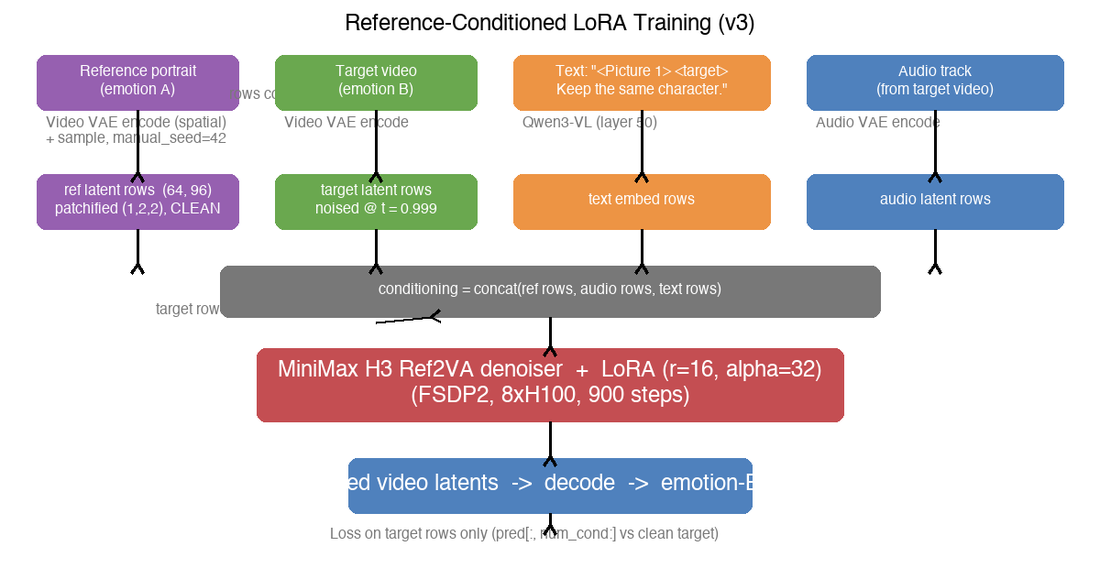
\includegraphics[width=\columnwidth]{paper_figure2.png}
\caption{Reference-conditioned training layout. The reference portrait is encoded with the video
autoencoder (sampled, seed 42) and added \emph{clean} at $t=0.999$ alongside the target rows, which
are the only rows that receive noise and loss. Text/audio rows are unchanged from Ref2VA training.}
\label{fig:method}
\end{figure}

\textbf{Reference encoding (training).} We patch the cache builder to encode each reference image
with the video autoencoder exactly as at inference: cover-resize, spatial encode, \emph{sample}
the posterior under seed 42, round to float16 (matching the released model's conditioning),
normalize, and patchify into conditioning rows. Each training sample stores \texttt{ref\_video}
rows.

\textbf{Training layout.} We extend the packing so a reference block precedes the target rows
($[\text{text}\mid\text{reference}\mid\text{target audio}\mid\text{target video}]$), with the
reference rows fed \emph{clean} at timestep 0.999 (identical to inference conditioning) and the
loss computed \textbf{only on target rows}. Training sequences grow from 537 to $\approx$602 rows
(256$^2$) or $\approx$4698 rows (768$^2$).

\textbf{Data.} Twenty-two clips generated on a single $8\times$H100 node: (a) $10$
\emph{preservation} clips, each pairing a distinct character's portrait (actors a01/a02/a03/a07/
a09/a11/a16/a18/a21/a24) with its own base-generated clip, reference and target sharing the emotion;
(b) $12$ \emph{cross-emotion} pairs for character 1534125952 (portraits angry/joyful/sad/surprised),
where the reference shows emotion A but the target video (and prompt) express emotion $B\neq A$. The
cross-emotion pairs are the key supervision for ``prompt overrides reference.'' Training therefore
spans $10$ distinct characters for preservation plus one character for the cross-emotion signal; the
$8$ evaluation tasks use $7$ \emph{different} character references (Sec.~6.1), and the two tasks
whose reference (actor a15, character 1537882489) is \emph{absent} from training are exactly the
tasks where v3 generalizes (x01 2/2, x02 1/8 including the sad breakthrough, Sec.~6.2).

All training is LoRA rank 16 / alpha 32, 900 steps, 8$\times$H100 with DeepSpeed-ZeRO-3
($\sim$15--80 min per run depending on resolution).

\section{Experiments}
\subsection{Setup}
Models: base; LoRA-v1 (9 clips, 300 steps); LoRA-v2 (18 clips, 600 steps); \textbf{LoRA-v3
(reference-conditioned, 22 clips, 256$^2$, 900 steps)}; LoRA-v4 (reference-conditioned, same 22
clips, \textbf{768$^2$}, 900 steps)---the v3/v4 pair isolates training resolution. Inference:
768$\times$768$\times$124, 16 steps, seeds 42 \& 1234, judge on 8 frames. Success: judged emotion
== target. The eight tasks use seven distinct character references (a01/a02/a03/a07/a11/a15/a18,
Table~1); a15 (tasks x01, x02) does not appear in the training set (Sec.~5), so x01/x02 double as
unseen-character generalization probes.

\subsection{Main results}
Per-task success across seeds is in the release together with full verdicts and confidences; the
matched base-vs-v3 comparison is Table~\ref{tab:matched}. We do not tabulate the older unmatched
per-model counts here: their denominators differ by task, which is precisely the defect Finding~B
corrects.



Figure~\ref{fig:qual} shows one representative frame per task for the base model and our
reference-conditioned LoRA-v3, together with the Qwen2-VL judge verdicts. The neutral$\rightarrow$sad
row is the headline: base is judged neutral while v3 is judged sad under an otherwise identical
generation.

\begin{figure*}[t]
\centering
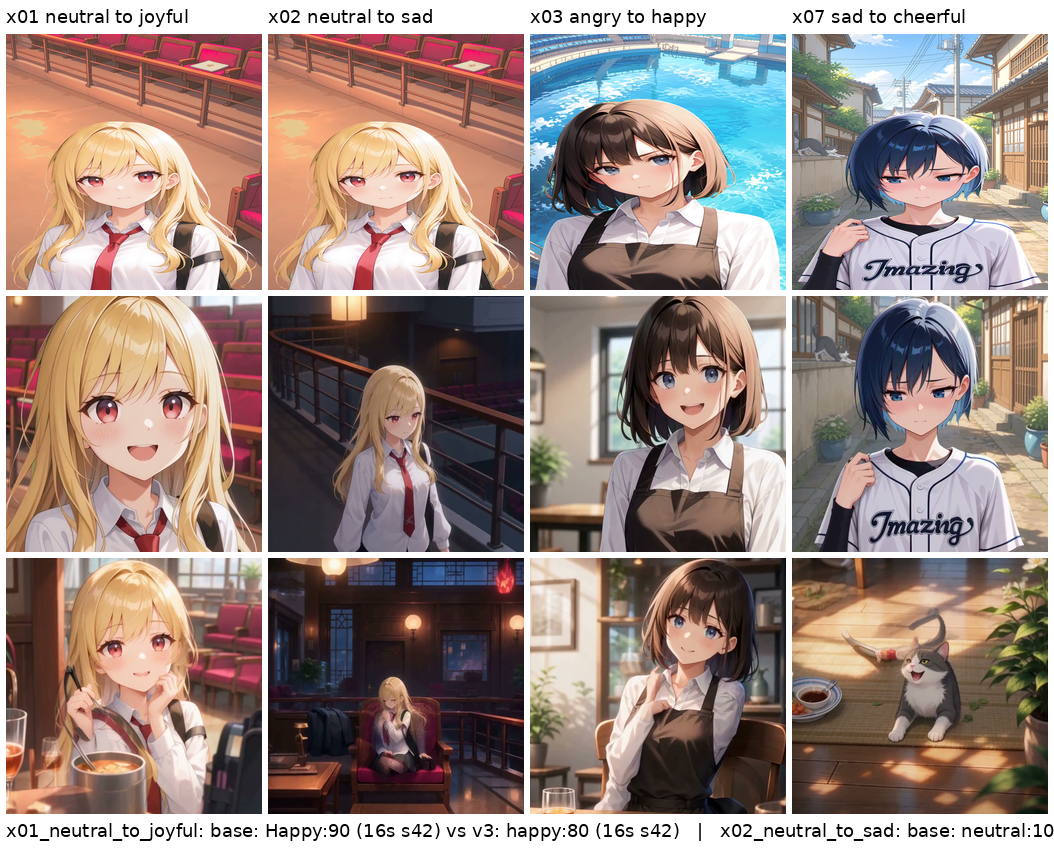
\includegraphics[width=\textwidth]{paper_figure1.png}
\caption{\textbf{Qualitative comparison (16 steps, 8-frame judge).} Columns are tasks (reference
portrait shown in the top row); rows are the reference, the base model, and our
reference-conditioned LoRA-v3. Judge verdicts (15-class, base vs v3): x01 neutral 50 vs happy 80;
x02 \textbf{neutral 100 vs sad 80} (the controlled negative-emotion demonstration, Finding~A); x03
happy 90 vs neutral 100; x07 neutral 50 vs happy 80.}
\label{fig:qual}
\end{figure*}

\textbf{Finding A --- the decisive cell is scoring-dependent, and its control does not hold.} Task
x02 (neutral$\rightarrow$sad) is the only negative target ever scored as a hit: v3 is judged
\textbf{sad (80)} at seed 1234---one of eight seeds (1/8)---and, under the primary protocol, base is
never sad across seven seeds (0/7). The 1/8 vs 0/7 difference is not significant (Fisher exact
$p{=}1.00$; overlapping Clopper--Pearson intervals) and rests on a single generation per model,
precisely the single-configuration evidence we warn against. It is also scoring-dependent along
every axis of Sec.~4.1 (Table~\ref{tab:judges}): Qwen2-VL says sad:80 and Qwen3.8-27B independently
sad:85/82 while Qwen3-VL-32B dissents (worried:85); that dissent flips to sad when the option list is
merely reversed; an 8-frame montage flips v3 to neutral; and, decisively, the base control fails
under full-clip scoring, where base x02 is judged sad at 2/6 seeds by both re-scored judges. Both
dissenters also mislabel a clear crying portrait ``surprised'' while Qwen3.8-27B reads it fearful:85,
so the static check fails for every judge (0/5). We present x02 not as an effect but as the clearest
illustration of the thesis: a cell whose verdict moves with the judge, the option order and the
frames judged, and whose control premise dissolves once the whole clip is scored. (LoRA-v4, 768$^2$,
reproduces the seed-1234 verdict and x02's reference is unseen in training; both facts concern the
cell, not the claim.) \begin{table}[!t]
\centering\scriptsize
\caption{Four open VLM judges, same 15-class protocol and frames, on the 17 known-emotion portraits
whose labels are inside the 15-class taxonomy (identical set for all four). Sanity strict = exact
match; sanity lenient applies the paper's synonym rule (joyful/cheerful/happy one family). None
passes, and \emph{no judge recognizes any negative emotion} (sad/angry/worried/anxious/disgusted:
0 for all four). On a clear crying portrait, the dissenters answer ``surprised'' and the
corroborating Qwen3.8-27B answers ``fearful''---no judge is validated for sad. Base x02 is neutral
under all four; v3 x02 is sad under Qwen2-VL and Qwen3.8-27B. Verdicts parsed as the last WORD:SCORE in each raw response (released).}
\label{tab:judges}
\setlength{\tabcolsep}{3pt}
\begin{tabular}{@{}lccccc@{}}
\toprule
Judge & s. strict & s. len. & v3 x02 & base x02\\
\midrule
Qwen2-VL-7B & 1/17 & 4/17 & \textbf{sad 80} & neutral 50\\
Qwen2.5-VL-7B & 0/17 & 5/17 & neutral 85 & neutral 95\\
Qwen3-VL-32B & 1/17 & 6/17 & worried 85 & neutral 95\\
Qwen3.8-27B & 0/17 & 7/17 & \textbf{sad 82} & neutral 78\\
\bottomrule
\end{tabular}
\end{table}



\textbf{Finding B --- we retract the task-level claim: a matched experiment shows no effect.} Our earlier
comparison was not task-matched: the base model had 16-step clips for only 4 of the 8 tasks
(x01/x02/x03/x07), so any aggregate over the 88-config pool---which also contains reference-swap probes,
an x02 seed sweep and non-16-step rows---mixes task composition into the ``success rate.'' Prompted by the
frame-span result, we therefore ran the experiment that comparison lacked: the base model regenerated on
\textbf{all 8 tasks at both seeds}, 16 steps, inference settings identical to the v3 evaluation, judged
with the same 15-class protocol. That gives 16 fully paired cells per judge (Table~\ref{tab:matched}).
All four judges return a null result and the strongest scores the base \emph{higher}: base 4/16 vs
v3 6/16 (Qwen2-VL, Fisher $p{=}0.70$, exact paired McNemar $p{=}0.69$), 6/16 vs 6/16 (Qwen2.5-VL,
$p{=}1.00$ both tests), 9/16 vs 8/16 (Qwen3-VL-32B, $p{=}1.00$ both tests) and 8/12 vs 8/12
(Qwen3.8-27B on the 12 cells it parses, $p{=}1.00$ both tests).

Two cells of that matrix independently falsify premises our earlier reading depended on, under the
primary 0--1\,s protocol and with no appeal to frame span: \textbf{base x02 at seed 42 is judged sad} by
Qwen3-VL-32B (so ``the base never expresses sad'' was an artifact of the base arm having a single x02
clip), and \textbf{base x08 at seed 1234 is judged angry} by both Qwen2-VL and Qwen3-VL-32B (so the
frown-type boundary of Finding~C is not a wall the base model cannot pass). Re-scoring the older 4-task
clips over the full duration (Sec.~4.1) points the same way---both arms end level at 3/4---but is now
secondary, because the paired matrix measures the effect directly and finds none. We therefore retract the
task-level claim entirely: the reference-conditioned LoRA produces \textbf{no measurable task-level
improvement} in emotion control, and the appearance of one came from an unmatched comparison scored over
the opening second of each clip. What it does change is the mechanism (Finding~D).

\begin{table}[!t]
\centering\small
\caption{Fully paired base-vs-v3 matrix: base regenerated on all 8 tasks at both seeds under the v3
inference settings (16 steps, 768$^2$, 124 frames), same 15-class protocol, 16 paired cells per judge,
exact tests. All four judges are null; the strongest scores the base higher.
$^{*}$Qwen3.8-27B parses 12 of the 16 cells.}
\label{tab:matched}
\begin{tabular}{@{}lcccc@{}}
\toprule
Judge & base & v3 & Fisher & McNemar\\
\midrule
Qwen2-VL-7B    & 4/16 & 6/16 & 0.70 & 0.69\\
Qwen2.5-VL-7B  & 6/16 & 6/16 & 1.00 & 1.00\\
Qwen3-VL-32B   & \textbf{9/16} & 8/16 & 1.00 & 1.00\\
Qwen3.8-27B$^{*}$ & 8/12 & 8/12 & 1.00 & 1.00\\
\bottomrule
\end{tabular}
\end{table}


\textbf{Inter-judge agreement (quantified).} Sweeping all 88 clip-configs through all four judges under
the identical protocol gives high agreement \emph{within} a capability tier---71.6\% for the two 7B
models (Qwen2-VL vs Qwen2.5-VL, Cohen $\kappa{=}0.49$) and 68.8\% for the two newest (Qwen3-VL-32B vs
Qwen3.8-27B, $\kappa{=}0.63$)---but only 41.6--47.7\% \emph{across} tiers; just 23 of 77 fully covered
configs are unanimous (Fleiss $\kappa{=}0.38$; 33/77 and 0.48 under the synonym rule). Disagreement
therefore scales with generation and size rather than being random noise, and it is concentrated on
\emph{whether} an emotion is present: dropping configs that both judges call neutral leaves only
36.7--50.0\% agreement, yet where both commit to a non-neutral emotion they agree 87.9--100\%. The
failure mode is a difference in neutrality threshold, not label confusion.

\textbf{The judges are not even stable against option order.} Holding the judge, the frames and greedy
decoding fixed and merely \emph{reversing the order of the 15 answer options} changes 17/88 verdicts for
Qwen2-VL (self-agreement 80.7\%, $\kappa{=}0.65$) and 10/88 for Qwen3-VL-32B (88.6\%, $\kappa{=}0.86$);
a duplicate run of the same configuration reproduces 88/88 labels, so this is a property of the prompt,
not sampling noise. The flips land on decision-relevant cells: the base x01 clip flips
neutral$\rightarrow$happy (so a baseline ``failure'' becomes a success), and Qwen3-VL-32B's dissent on
the decisive v3 x02 clip flips worried$\rightarrow$sad. This is the strongest single piece of evidence
that the evaluation, not the model, is the bottleneck.

\textbf{Finding C --- frown-type targets are untestable with the weakest judge.} Worried (x04) and
angry (x08) are \emph{never emitted} by Qwen2-VL (which uses only 4 of 15 classes over 88 configs),
so their failure cannot be attributed to the model with that judge---this is a boundary of our
\emph{evaluation}, not (only) of the model. Qwen3-VL-32B (9/15 classes) and Qwen3.8-27B judge the v3
x04 clip \emph{worried} (95 and 80), unlocking the cell; x08 stays neutral. Both newer judges also
read a subtle known-sad portrait as worried, so x04 is a success with a caveat, not clean validation;
a 768$^2$ training-resolution variant (v4, matching the eval layout) never yields these classes,
ruling out a layout-mismatch explanation. Judge sensitivity to frown-type emotions remains
unverified.

\textbf{Finding D --- direct evidence for reference-emotion dominance and its suppression.}
Table~\ref{tab:mechanism} holds the prompt fixed (``She looks sad.'') and varies the reference
emotion (four portraits of one character, both seeds). Within the judge's reliable vocabulary the
base output tracks the \emph{reference}---sad 2/2, surprised 2/2, joyful 1/2 (5/8) under Qwen2-VL
and 4/8 under Qwen3-VL-32B at 0--1\,s---the reference overrides the prompt, confirming the root cause
we hypothesize. This is the one claim that survives every scoring we tried: under full-clip
re-scoring the base still tracks the reference (3/8 and 4/8) while v3 stays decoupled (2/8) in all
four judge$\times$frame-span conditions; under a $\ge$2-of-3 majority consensus base tracks 4/8 vs
v3 2/8 with two discordant pairs, both favouring suppression (exact McNemar $p{=}0.50$; Qwen2-VL alone
gives three discordant pairs, $p{=}0.25$; underpowered at $n{=}8$ either way). We therefore read it as a consistent direction, not an
established effect, and we cannot rule out that part of it is a regression toward neutral (v4's
all-neutral behavior at seed 42 is a caution). Target rendering under v3 is partial at best.

\begin{table*}[!t]
\centering\small
\caption{Reference-swap test, prompt fixed ``She looks sad.'' (15-class judge, 16 steps, 8
frames). Base tracks the reference on the judge's reliable classes (sad/surprised both seeds,
joyful one); v3 decouples (mostly neutral). The angry reference is never emitted as angry by the
judge.}
\label{tab:mechanism}
\begin{tabular}{@{}lccccc@{}}
\toprule
Reference & base s42 & base s1234 & v3 s42 & v3 s1234\\
\midrule
angry & sad 80 & neutral 50 & neutral 100 & neutral 50\\
joyful & neutral 50 & \textbf{happy 80} & neutral 50 & neutral 100\\
sad & \textbf{sad 80} & \textbf{sad 80} & sad 80 & sad 80\\
surprised & \textbf{surprised 80} & \textbf{surprised 100} & neutral 50 & neutral 100\\
\bottomrule
\end{tabular}
\end{table*}

\subsection{Identity-consistency analysis}
A central promise of portrait-reference generation is identity preservation. We quantify it two
ways. \textbf{(i) CLIP cosine similarity} (ViT-L/14) between the reference portrait and three
frames (early/middle/late) of each generated clip, averaged (Table~\ref{tab:identity}). The metric
is seed-stable (mean $|\Delta|$ across seeds 42/1234 is 0.078, and $\le$0.10 for 5/8 tasks). Two
conclusions: base preserves identity slightly better than LoRA-v3 on shared tasks (0.80 vs 0.73
average), i.e. our intervention trades a small amount of identity fidelity for emotion control; and
identity is \emph{not} uniformly strong---x07 s42 (0.585) and x08 s1234 (0.579) are the lowest,
both being tasks where the target emotion was most visibly rendered. \textbf{(ii) A binary
Qwen2-VL check} (``same character?'', single middle frame) as a sanity signal. Its verdicts flip
across seeds for 6/8 tasks, so we treat it as qualitative only; where it disagrees with CLIP (x01
at seed 1234: VLM NO vs CLIP 0.775), we trust the continuous, seed-stable CLIP score. Both metrics
agree on the direction of the emotion--identity tradeoff: the model pays for expression change with
identity deviation. A dedicated face-embedding identity metric is future work.

\begin{table*}[t]
\centering\small
\caption{Identity preservation vs the reference portrait. Left: CLIP ViT-L/14 cosine similarity
(mean over 3 frames), higher is better; base is the 16-step model (seed 42 for x01/x03, seed 1234
for x02/x07). LoRA-v3 trades a small amount of identity fidelity for emotion control (0.73 vs 0.80
average on shared tasks). Right: binary Qwen2-VL ``same character?'' verdicts (seed 42 / seed 1234);
flips indicate this single-frame signal is qualitative only.}
\label{tab:identity}
\begin{tabular}{@{}lccccc@{}}
\toprule
 & \multicolumn{3}{c}{CLIP similarity} & \multicolumn{2}{c}{Qwen2-VL (s42/s1234)}\\
\cmidrule(lr){2-4}\cmidrule(lr){5-6}
Task & base & v3 s42 & v3 s1234 & verdict & same?\\
\midrule
x01 neutral$\rightarrow$joyful & 0.730 & 0.767 & 0.775 & YES / NO & flip\\
x02 neutral$\rightarrow$sad & 0.819 & 0.694 & 0.700 & NO / YES & flip\\
x03 angry$\rightarrow$happy & 0.826 & 0.808 & 0.771 & YES / YES & stable\\
x04 joyful$\rightarrow$worried & --- & 0.659 & 0.730 & NO / YES & flip\\
x05 amused$\rightarrow$surprised & --- & 0.808 & 0.754 & YES / YES & stable\\
x06 anxious$\rightarrow$relieved & --- & 0.831 & 0.730 & YES / NO & flip\\
x07 sad$\rightarrow$cheerful & 0.838 & 0.585 & 0.758 & NO / YES & flip\\
x08 curious$\rightarrow$angry & --- & 0.755 & 0.579 & YES / NO & flip\\
\bottomrule
\end{tabular}
\end{table*}

\subsection{Ablation: training resolution (v3 vs v4)}
We trained the reference-conditioned LoRA at both 256$^2$ (v3) and 768$^2$ (v4) on identical data.
Contrary to the ``layout mismatch'' hypothesis, 768$^2$ training is \emph{worse}: v4 scores 0/8 at
seed 42 (all neutral) and 2/8 at seed 1234, versus v3's 3/8 and 4/8; the previously robust positive
tasks x01/x03 regress to neutral. v4's training loss is \emph{lower} (0.30 vs 0.45) yet its
behavior is worse---consistent with overfitting on 22 clips at higher resolution with a fixed-rank
LoRA spread over $\sim$8$\times$ more sequence. This rules out resolution as the bottleneck and
is consistent with the capacity reading of Finding~C.

\section{Limitations}
\begin{itemize}
\item \textbf{Scale.} Training uses only 22 clips: 10 preservation clips spanning 10 characters
plus 12 cross-emotion pairs for a \emph{single} character. The emotion-transfer (cross-emotion)
supervision is single-character, and 7-8 emotion targets are never seen as targets in training;
larger multi-character cross-emotion corpora are needed for stronger claims. The evaluation's
multi-character reference coverage (7 characters, one unseen in training) mitigates but does not
remove this limitation.
\item \textbf{Evaluation is the weak link.} Four open VL judges (Qwen2-VL-7B, Qwen2.5-VL-7B,
Qwen3-VL-32B, Qwen3.8-27B) validate on 1/17, 0/17, 1/17, 0/17 of the same taxonomy-relevant
known-emotion portraits, with strong neutral/worried bias; the weakest never emits 11 of its 15
classes (worried/relieved/angry untestable with it); verdicts flip with seed, frame count, taxonomy,
judge choice, answer-option order, and---most strongly---judged frame span (Sec.~4.1). The frame-span
axis is also a temporal-coverage limitation of our primary protocol and of much prior practice: it
judged only the first second of each 5.2\,s clip, where the reference expression is most likely to
persist. The frame-span comparison covers 97 clips and three re-scored judges, and the mechanism test is
$n{=}8$; there is no human ground truth, so we can quantify the instability but not adjudicate it. A
human-study protocol is released as supplementary material.
\item \textbf{Identity.} Our CLIP-based identity metric (seed-stable, Sec.~6.4) shows a small
identity-for-emotion tradeoff, but a dedicated face-embedding metric with multi-frame aggregation
is needed before strong claims.
\item \textbf{Boundary.} Frown-type negative emotions remain unsolved; our evidence attributes
this to the judge and to LoRA capacity, not to an absolute limit: the base model reaches angry on x08.
\item \textbf{Audio.} All reported tasks use video-only judgment; joint audio+emotion control is
out of scope (audio is trained jointly but not evaluated for emotion).
\end{itemize}

\section{Conclusion}
We presented a reproducible study of emotion-controllable anime character video generation on MiniMax
H3 whose central lesson is that the evaluation, not the model, is the binding constraint.
Emotion-control evaluation here is not invariant to three essentially free protocol
choices---judge identity (only 23/77 configs unanimous; none of four judges validated on any negative
emotion), answer-option order (up to 19\% of verdicts flip on identical frames), and judged frame span
(up to 35\%, significant in three of six arm$\times$judge cells, McNemar $p{\le}0.021$). The third reverses our own results,
so we \emph{retract} the task-level claim for our reference-conditioned LoRA: over the whole clip the
baseline's ``failures'' become successes and its ``never-sad'' control fails, and no measurable
task-level improvement survives. What survives every scoring is the mechanism---the LoRA suppresses
reference-emotion tracking (base 5/8, 4/8, 3/8, 4/8 vs v3 2/8 across four judge$\times$frame-span
conditions), read as a consistent direction because it is underpowered ($n{=}8$; exact McNemar
$p{=}0.50$ on consensus labels, $p{=}0.25$ for the single most sensitive judge).
Frown-type targets remain untestable with the weakest judge, and a 768$^2$ resolution ablation rules
out a layout-mismatch explanation. Until judges are validated on the emotions they score and protocols
fix temporal coverage, reported emotion-control gains are not interpretable. All verdicts, frames and
analysis scripts are released.

\bibliographystyle{plainnat}
\begin{thebibliography}{99}
\bibitem[minimax2025]{minimax2025} MiniMax.
\newblock \emph{MiniMax H3: Open General Intelligence} (model release), 2025.
\newblock \url{https://www.minimax.io/news/minimax-h3-open-source}
\bibitem[Yang et~al.(2024)]{cogvideox2024} Q.~Yang et~al.
\newblock CogVideoX: Text-to-video diffusion models with an expert transformer.
\newblock \emph{arXiv:2408.06072}, 2024.
\bibitem[Tencent(2024)]{hunyuan2024} Tencent.
\newblock HunyuanVideo: A systematic framework for large video generative models.
\newblock \emph{arXiv:2412.03603}, 2024.
\bibitem[Wan Team(2025)]{wan2025} Wan~Team.
\newblock Wan: Open and advanced large-scale video generative models.
\newblock \emph{arXiv:2503.20314}, 2025.
\bibitem[OpenAI(2024)]{sora2024} OpenAI.
\newblock Video generation models as world simulators (Sora), 2024.
\bibitem[Hu(2023)]{animateanyone2023} A.~Hu.
\newblock Animate Anyone: Consistent and controllable image-to-video synthesis for character
animation. \emph{arXiv:2311.17117}, 2023.
\bibitem[Tian et~al.(2024)]{stableanimator2024} H.~Tian et~al.
\newblock StableAnimator: High-quality identity-preserving human image animation.
\newblock \emph{arXiv:2411.17697}, 2024.
\bibitem[Ye et~al.(2023)]{ipadapter2023} H.~Ye et~al.
\newblock IP-Adapter: Text compatible image prompt adapter for text-to-image diffusion models.
\newblock \emph{arXiv:2308.06721}, 2023.
\bibitem[Hu et~al.(2021)]{lora2021} E.~Hu et~al.
\newblock LoRA: Low-rank adaptation of large language models.
\newblock \emph{arXiv:2106.09685}, 2021.
\bibitem[Ruiz et~al.(2022)]{dreambooth2022} N.~Ruiz et~al.
\newblock DreamBooth: Fine tuning text-to-image diffusion models for subject-driven generation.
\newblock \emph{arXiv:2208.12242}, 2022.
\bibitem[Wang et~al.(2024)]{qwen2vl2024} P.~Wang et~al.
\newblock Qwen2-VL: Enhancing vision-language model's perception of the world at any resolution.
\newblock \emph{arXiv:2409.12191}, 2024.
\end{thebibliography}

\end{document}
